\gls{BLL} eller \gls{forretningslogik}ken indkapsler kassesystemets funktionalitet. Det er i \gls{BLL}, hvor salg behandles og håndteres. Dette skal ses i modsætning til \Gls{brugergraenseflade}n og \gls{DAL}, som ikke danner en mening af den data, de får ind. Forholdet kan ses i Figur~\ref{fig:bll}. Det gør \gls{BLL} derimod. \gls{BLL} sørger f.eks. for at et produkt bliver tilføjet til den igangværende ordre. Derfor kan \gls{BLL} ses, som en slags ''opskrift'' for hvordan data skal behandles og håndteres.

\begin{figure}[H]
	\centering
	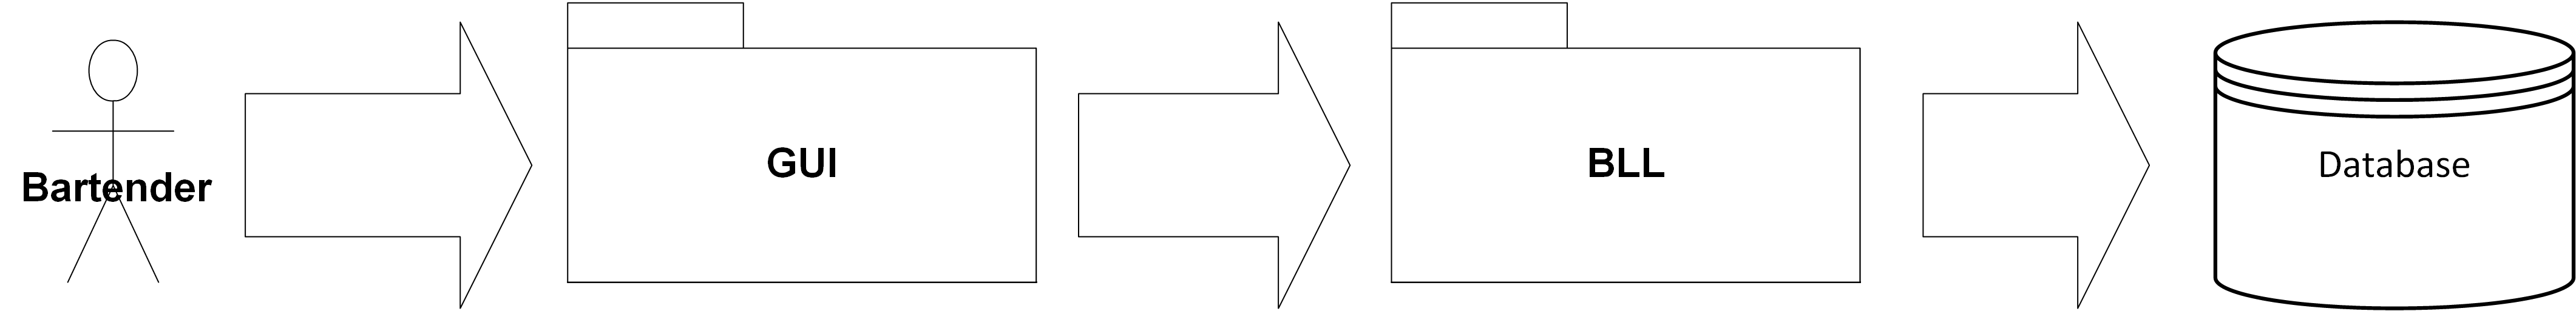
\includegraphics[width=0.8\textwidth]{Rapport/BLL.png}
	\caption{BLL i forhold til GUI og Databasen}
	\label{fig:bll}
\end{figure}

I underafsnittene vil de bemærkelsesværdige pakker i systemet beskrives. Det er de pakker, som er essentielle, for at systemet virker. Disse pakker er:
\begin{itemize}
	\item Orders
	\item Payment
	\item Sales
\end{itemize}

\subsubsection{Orders}
Ordre eller \textit{Order}'s varetages af pakken \texttt{Orders}. Her er en \textit{Order} en database model, som pakken kender til. Pakken \texttt{Orders} er opbygget, så den indeholder en \Gls{controller} og et \gls{Dao}. \Gls{controller}ens opgave er at styre alt logikken, som omhandler behandlingen af en \textit{Order}. Dvs. at \gls{controller}en skal stå for at oprette, tilføje produkter til og evt. nulstille en \textit{Order}. Når behandlingen er fuldført, skal ordren, sættes ind i databasen. Dette sker vha. \gls{Dao}. \gls{Dao}'s eneste opgave er at håndtere \textit{Order}'s i forhold til databasen. Dette indebærer at indsætte, hente og slette \textit{Order}'s i databasen.
\newline\newline
Når et produkt eller et \textit{Product} indsættes i en \textit{Order}, bliver der tilføjet en \textit{OrderLine} til en liste af \textit{OrderLine}'s, som ligger i \textit{Order} objektet. En \textit{OrderLine} indeholder et \textit{Product}, dets antal, dets pris pr. stk. og en evt. rabat eller \textit{Discount} med rabatten pr. stk. Derved sikres det at en ordre kan slås op i databasen med de eksakte priser samt evt. rabatter.

\subsubsection{Payment}
Transaktioner eller \textit{Transaction}'s varetages af pakken \texttt{Payment}. \texttt{Transactions} indeholder ligesom \texttt{Orders}, en \Gls{controller} og et \Gls{Dao}. Konceptet er det samme som i \texttt{Orders}. \Gls{controller}en skal holde styr på logikken og \Gls{Dao} skal sørger for, at \textit{Transaction}'s bliver skrevet i databasen.
\newline\newline
Da \textit{Transaction}'s kan foregå over flere platforme, skal \gls{controller}en have en liste af \textit{PaymentProvider}'s. En \textit{PaymentProvider}  beskriver en betalingsmetode. Klassen skal holde styr på omsætningen fra den pågældende betalingsmetode og hvilke funktioner i de pågældende \gls{API}, som de skal bruge for f.eks. at gennemføre en betaling. Dette gør sig selvfølgelig ikke gældende, når det er en \textit{CashPayment} eller kontantbetaling. Byttepengene varetages i \texttt{CashDrawer} eller pengeskuffen. \texttt{CashDrawer} holder styr på mængden af byttepenge, som gerne skulle være at finde i skuffen. Ved afstemning vil byttepengene bliver sat op imod omsætningen fra de forskellige \textit{PaymentProvider}'s for at sikre at byttepenge stemmer overens efter dagens salg.
\newline\newline
Når en \textit{Transaction} er udført skrives den til databasen via \gls{Dao}. En \textit{Transaction} skal pege tilbage til \textit{Order}. Så den resterende total af salget kan udregnes af \texttt{Orders} pakken.

\subsubsection{Sales}
\textit{Sales} står for at samle hele kassesystemet. Det er her, hvor funktionaliteten fra \texttt{Orders} og \texttt{Payment} sammenfattes og bruges til at skabe en større mening. \textit{Sales} står for at sende den rette information videre til de respektive pakker. F.eks. når der tilføjes et produkt til en \textit{Order}, skal dette videreformidles til \texttt{Order} pakken. Eller f.eks. hvis en \textit{Order} skal betales, skal betalingen videreformidles til \texttt{Payment} pakken.
\newline\newline
Ved at samle hele systemets funktionalitet i \texttt{Sales} betyder at vores \gls{brugergraenseflade} kun skal ''snakke'' med \texttt{Sales}. \Gls{brugergraenseflade}n behøves ikke at kende til al det underliggende og det behøver \texttt{Sales} i den forstand heller ikke.